\appendix
\addtocontents{toc}{\protect\setcounter{tocdepth}{1}}


\section{Supplementary Material}\label{sec:supplementary-material}

\subsection{Data sources, availability and additional details}\label{sec:data-sources-availability-and-additional-details}

Survey regions and country borders were retrieved from the Spatial Data Repository \autocite{icfinternationalSpatialDataRepository2022} and the Database of Global Administrative Boundaries (GADM) \autocite{globaladministrativeareasGADMDatabaseGlobal2022}. The remotely sensed covariates in \autoref{sec:geographic-malaria-risk-in-mali} are mean values over the year preceding the start date of the survey fieldwork. All raster files are open-access and were retrieved from the Google Earth Engine API \autocite{gorelickGoogleEarthEngine2017} or the respective provider as described in the respective publications at a spatial resolution of 1km x 1km. 

To create a fine-scaled country grid I use the spatial unit indexing system \textit{H3: A Hexagonal Hierarchical Geospatial Indexing System} \autocite{ubertechnologiesH3HexagonalHierarchical2022}. The grid level estimates are produced for a grid of resolution 7, hexagons with an area of approximately 5km$^2$. I extract for each cluster location or hexagon centroid the value interpolated from the values of the four nearest raster cells. One exception is the population data, where exact areal extraction is used to obtain a consistent disaggregation of population totals. 


\subsection{Computational implementation}\label{sec:computational-implementation}

All analyses were conducted in {\tt R} 4.2.2 \autocite{rcoreteamLanguageEnvironmentStatistical2022} and Python 3.9.13. The code files and data requirements to fully replicate this work along with additional results are included in the corresponding GitHub repository.\footnote{See \url{https://github.com/danielseussler/ssahealthriskfactors}.}

The described models were fitted using the {\tt mboost} and {\tt gamboostLSS} packages \autocite{hothornMboostModelBasedBoosting2022, hofnerGamboostLSSPackageModel2016}, see also \textcite{hothornModelbasedBoosting2010} for an introduction. The following {\tt R} packages provided helpful functions for evaluation metrics, raster extraction and survey data analysis: \textcite{hamnerMetricsEvaluationMetrics2018, pfefferMalariaAtlasInterfaceGlobal2018, watsonRdhsPackageInteract2019, lumleySurveyAnalysisComplex2020, hijmansGeodataDownloadGeographic2022, bastonExactextractrFastExtraction2022}. 


\subsection{Distributions}
\label{appendix_distributions}

\subsubsection*{Binomial distribution}

\begin{equation*}
	Y \sim \: \Binomial(n, \mu)
\end{equation*}

For $y = 0, 1, \dots, n$ and $0 < \mu < 1$, the probability density function of the binomial distribution is 
\begin{equation}
	f(y \vert n, \mu) = \frac{n!}{y! (n-y)!} \mu ^y (1 - \mu)^{n-\mu}
\end{equation}
where the first and second moments are
\begin{align*}
	E(Y) &= n\mu, \\
	Var(Y) &= n \mu (1-\mu).
\end{align*}


\subsubsection*{Beta-binomial distribution}

\begin{equation*}
	Y \sim \: BB(n, \mu, \sigma)
\end{equation*}

For $y = 0, 1, \dots, n$, $0 < \mu < 1$, and $\sigma > 0$, the probability density function of the beta-binomial distribution is 
\begin{equation}
	f(y \vert n, \mu, \sigma) = \frac{\Gamma(n + 1)}{\Gamma(y + 1) \Gamma(n - y + 1)}
	\frac{
		\Gamma(\frac{1}{\sigma}) \Gamma(y + \frac{\mu}{\sigma}) \Gamma(n + \frac{(1-\mu)}{\sigma} - y)
	}{
		\Gamma(n + \frac{1}{\sigma}) \Gamma(\frac{\mu}{\sigma}) \Gamma(\frac{1-\mu}{\sigma})
	}.
\end{equation}
The corresponding first and second moments are 
\begin{align*}
	E(Y) &= n \mu, \\
	Var (Y) &= n \mu ( 1- \mu ) [ 1 + \sigma (n - 1) / (1 + \sigma) ].
\end{align*}
See also \textcite{rigbyDistributionsModelingLocation2019} for further information.



\subsection{Additional Results}\label{sec:additional-results}

In this section, I present additional figures and tables for the two case studies.

% latex table generated in R 4.2.2 by xtable 1.8-4 package
% Thu Jan 12 14:45:15 2023
\begin{table}[!p]
	\centering
	
	\begin{tabularx}{0.8\textwidth}{Xl}
		
		Base-learner & Frequency \\ \arrayrulecolor{black!30}\midrule
		cage & 1.00 \\ 
		csex & 1.00 \\ 
		ctwin & 1.00 \\ 
		cbord & 1.00 \\ 
		mbmi & 1.00 \\ 
		mage & 0.74 \\ 
		medu & 1.00 \\ 
		memployed & 0.22 \\ 
		mreligion & 0.98 \\ 
		nodead & 0.86 \\ 
		hmembers & 1.00 \\ 
		watersource & 0.90 \\ 
		sanitation & 0.44 \\ 
		wealth & 1.00 \\ 
		electricity & 0.30 \\ 
		radio & 1.00 \\ 
		television & 1.00 \\ 
		bicycle & 0.28 \\ 
		motorcycle & 0.82 \\ 
		car & 0.70 \\ 
		urban & 0.52 \\ 
		healthaccess & 0.36 \\ 
		cityaccess & 1.00 \\ 
		fews & 0.86 \\ 
		f(cage) & 1.00 \\ 
		f(mage) & 0.90 \\ 
		f(mbmi) & 0.40 \\ 
		f(medu) & 1.00 \\ 
		f(hmembers) & 0.48 \\ 
		f(healthaccess) & 0.68 \\ 
		f(cityaccess) & 0.98 \\ 
		f(dhsregion) & 1.00 \\ 
	\end{tabularx}

	\caption{Childhood malnutrition in Madagascar: selection frequencies of base learners over the 50 replications. The name indicates the linear effect only, f($\cdot$) is the non-linear deviation from the linear effect.}
	\label{tab:madagascar_selectionfreq}

\end{table}


\begin{figure}[!p ]
	\centering
	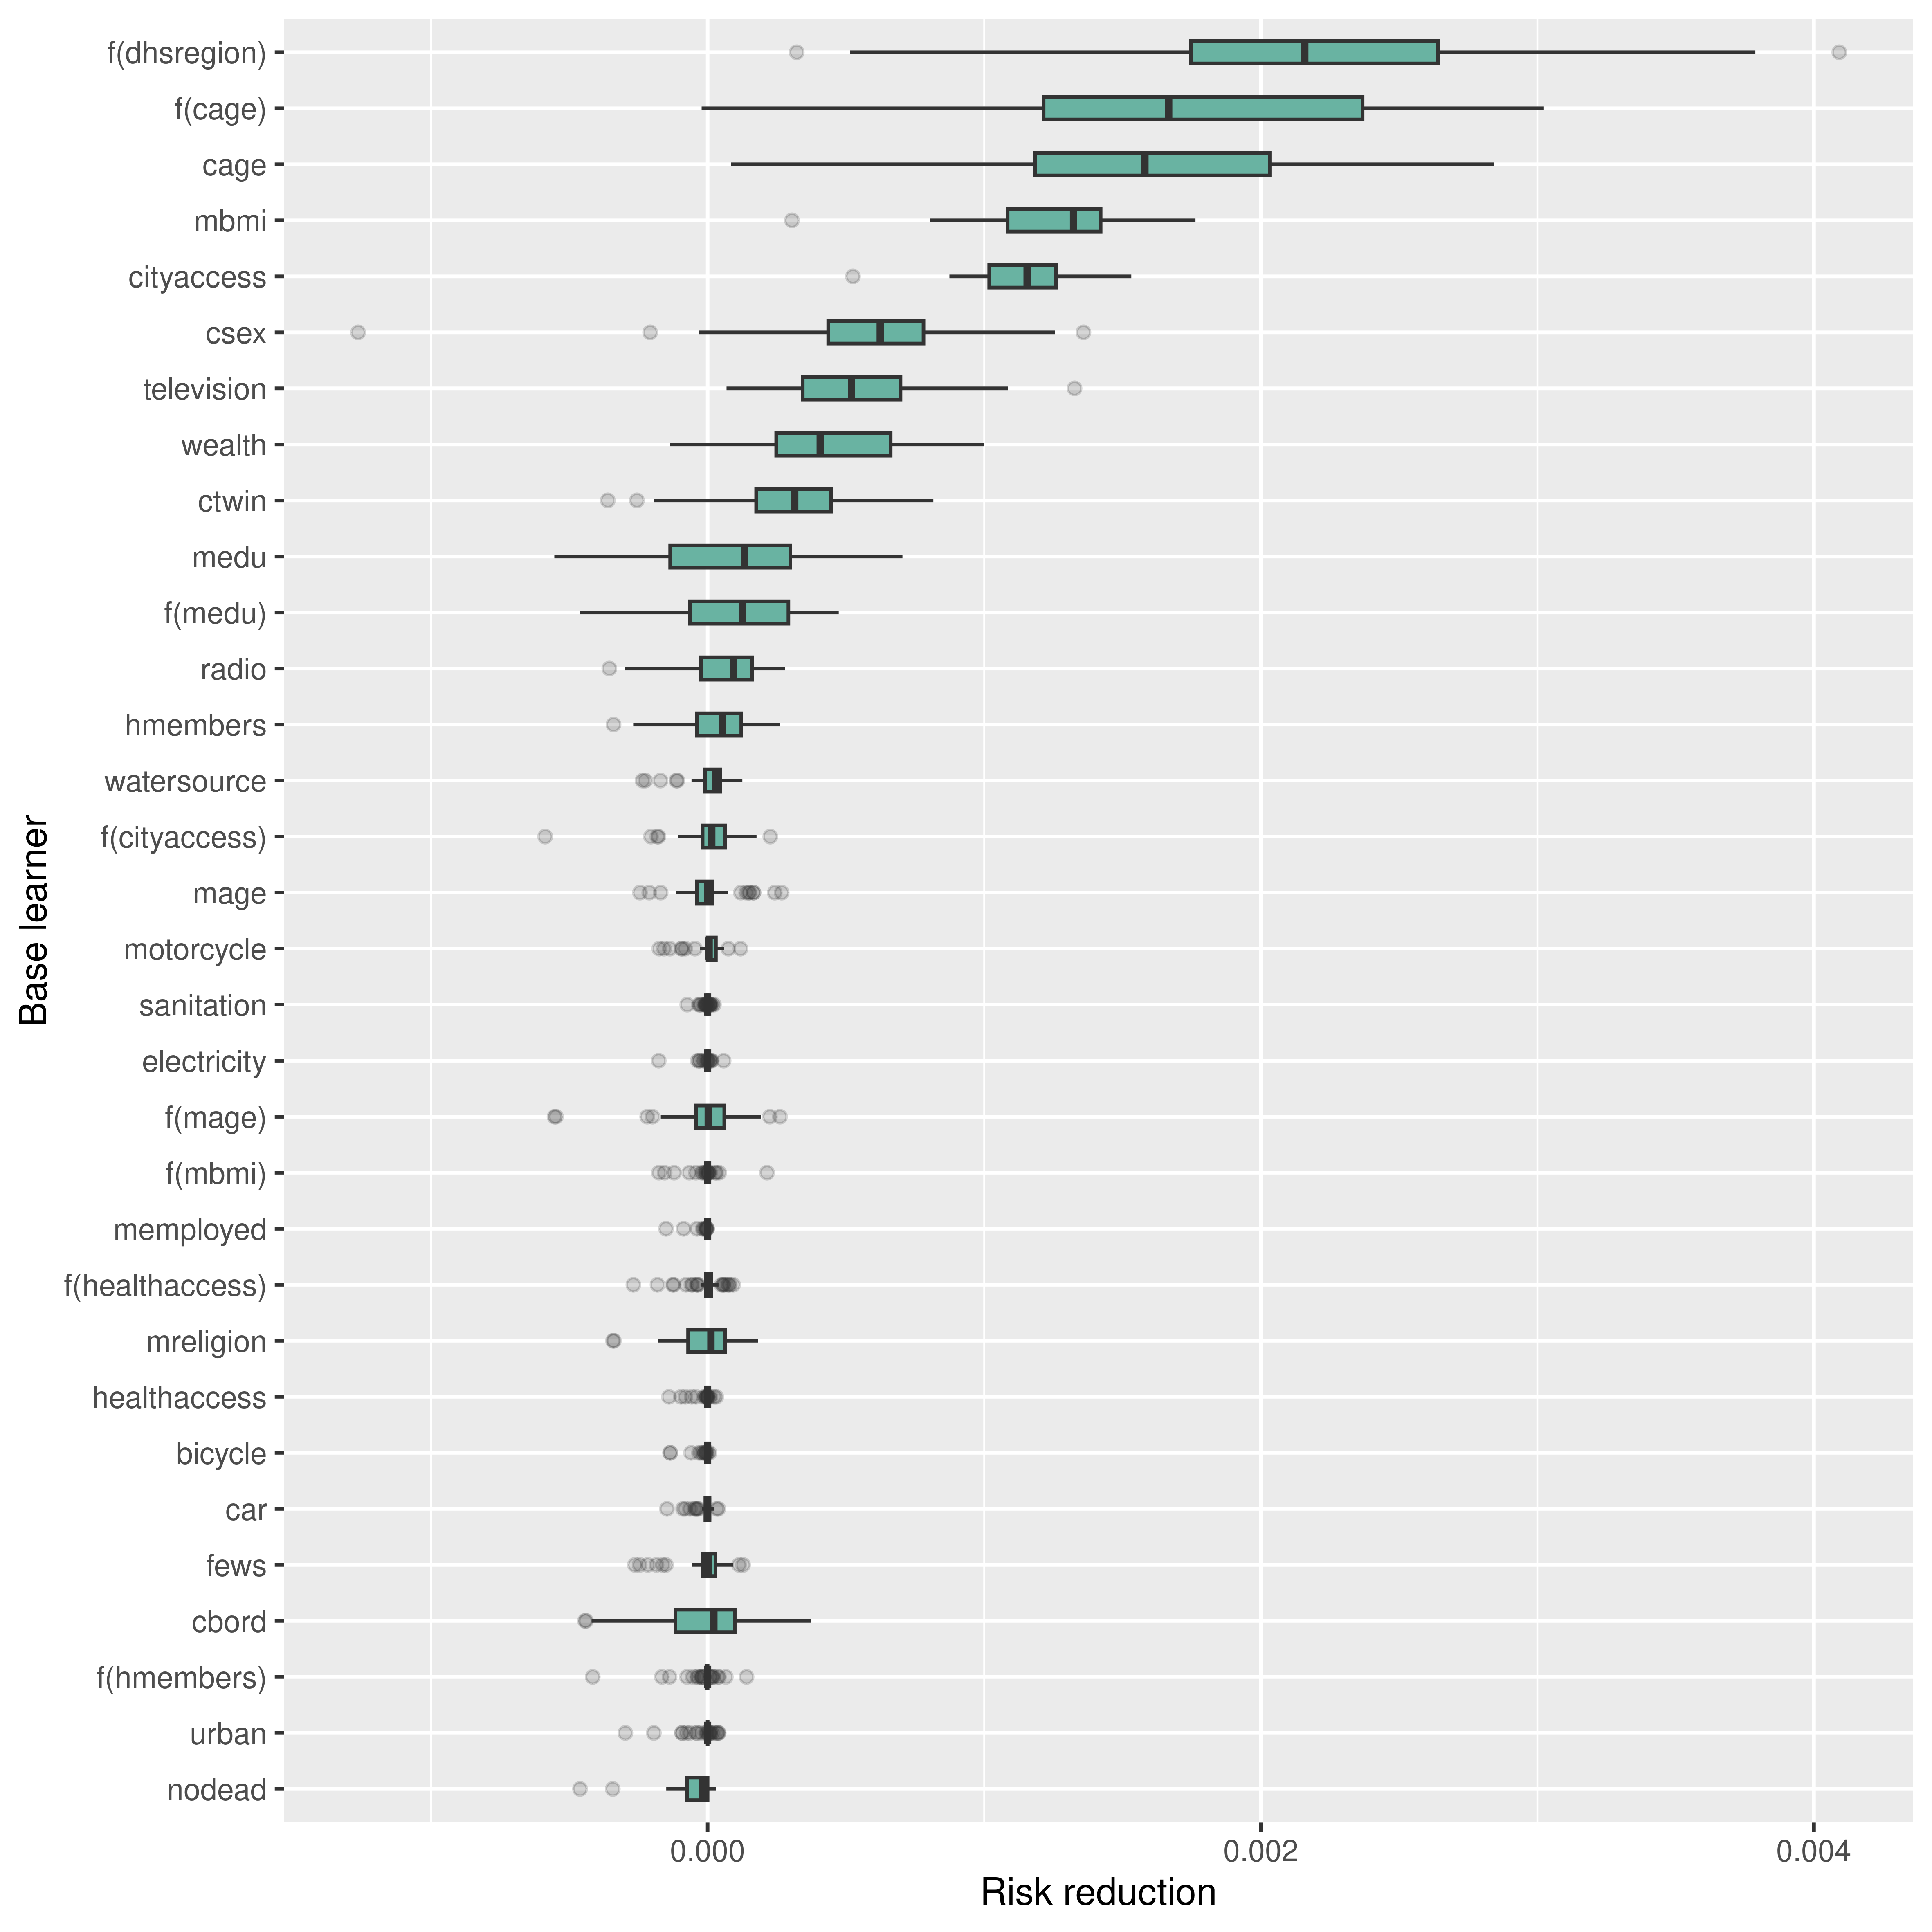
\includegraphics[width=0.9\textwidth, keepaspectratio]{figures/madagascar_variableimportance.png}
	\caption{Childhood malnutrition in Madagascar: empirical distributions of the variable importance of each base-learner by attributed risk reduction over 50 replications. Note, (small) negative risk reduction can be obtained as a fitting artefact if boosting iterations are extended beyond the maximum likelihood estimates.}
	\label{fig:madagascar_variableimportance}
\end{figure}

\begin{figure}[!p]
	\centering
	\includegraphics[width=0.9\textwidth, keepaspectratio]{figures/mali_predictionuncertainty.png}
	\caption{Geographic malaria risk in Mali: lower, upper quantiles and standard error of the predicted risk $\hat{\mu}$ based on 50 bootstrap samples.}
	\label{fig:mali_predictionuncertainty}
\end{figure}
